\input{tex/preamble_article.tex}
\begin{document}
\input{tex/forside.tex}
\newpage
\tableofcontents
\thispagestyle{empty}
\setcounter{page}{0}
\newpage
\section{Introduction}
The goal of this assignment is to implement sequential versions of two iterative ODE solvers, namely the Jacobi method and the Gauss-Seidel method. The Jacobi method is parallelized using openMP and the scalability is compared to the parallelization of the calculation of the Mandelbrot set. Finally a method for parallelizing the Gauss.Seidel method is discussed but not implemented.

\subsection{Computing Specifications}
Unless otherwise stated a lot of the specifications are fixed throughout the report. The code is written in C and compiled with the Sun Studio compiler. All the experiments are run on the hpcintro queue on a single node with one processors per node (ppn), which is specified in the submit.sh script. All the nodes on the cluster are identical, and the full specifications are given in talbe \ref{tab:spec}.
\begin{table}
\centering
\begin{tabular}{l l}
Architecture:     &     x86\_64 \\ \hline
CPU op-mode(s):    &    32-bit, 64-bit\\ \hline
Byte Order:         &   Little Endian\\ \hline
CPU(s):             &   20\\ \hline
On-line CPU(s) list:&   0-19\\ \hline
Thread(s) per core: &   1\\ \hline
Core(s) per socket: &   10\\ \hline
Socket(s):          &   2\\ \hline
NUMA node(s):       &   2\\ \hline
Vendor ID:          &   GenuineIntel\\ \hline
CPU family:         &   6\\ \hline
Model:              &   63\\ \hline
Stepping:           &   2\\ \hline
CPU MHz:            &   2601.000\\ \hline
BogoMIPS:           &   5187.68\\ \hline
Virtualization:     &   VT-x\\ \hline
L1d cache:          &   32kB\\ \hline
L1i cache:          &   32kB\\ \hline
L2 cache:           &   256kB\\ \hline
L3 cache:           &   25600kB\\ \hline
NUMA node0 CPU(s):  &   0-9\\ \hline
NUMA node1 CPU(s):  &   10-19\\
\end{tabular}
\caption{Table of the full machine specifications.}
\label{tab:spec}
\end{table}


\section{Assignment}
\subsection{Nat}

First, the goal is to write a native function, which performs a matrix-matrix multiplication. The shape has to be suitable for the operation, but it is arbitrary within the limits. We chose the native way, where the matrix is described using double pointers, i.e. A[i][j]. The choice of function prototypes and driver therefore follows.  \\
The general function prototype used is displayed below:
\begin{lstlisting}[language=C++, caption=Function Prototype]
void matmult_NNN(int m, int n, int k, double ** A, double ** B, double ** C)
\end{lstlisting}


\subsection{The Permutations}

Since the algorithm consists of three nested loops iterating over the three dimensions m, n and k, it is clear through basic combinatorics, that there is 3! = 6 possible ways to order the loops:\\
mnk - mkn - kmn - knm - nmk - nkm \\
The 6 permutations are implemented as separate functions in the library with names matmult\_NNN. The functions are obviously very similar to the already described nat function, but the function are however displayed below:

\begin{lstlisting}[language=C++, caption=lib]
void matmult_mkn(int m, int n, int k, double ** A, double ** B, double ** C){
	for(int i = 0; i < m;i++){
		for(int j = 0; j < n;j++){
			C[i][j] = 0;		
		}
	}


	for(int i = 0; i < m;i++){
		for(int l = 0; l < k;l++){
			for(int j = 0; j < n;j++){
				C[i][j] += A[i][l]*B[l][j];
			}
		}
	}
}
\end{lstlisting}

Here, the C matrix is defined in an earlier loop. The mkn permutation is here shown, since it will also turn out to be an important permutation throughout this report.
\subsection{Comparing the permutations}
The performance of the six different functions resulting from the possibilities of permuting mnk are tested with square matrices with memory footprints ranging from a few kB to hundreds of MB. The results are seen in figure \ref{fig:comp1} with compiler option $\mathrm{-fast}$ enabled. The performance of the six functions behave in pairs depending on the last index which corresponds to the innermost for-loop. The functions pair up depending on this index because it is the loop being executed the most times, and so any performance issue coming from this loop is executed the most times as well. As seen in the figure \ref{fig:comp1}, the permutations with $m$ as the last index is a factor of $\sim 2$ slower than the other four permutations for memory footprints smaller than L2 cache. This is because $m$ is the column size of matrices $A$ and $C$, so by having the $m$ loop as the innermost loop, a lot of cache misses will happen due to C being a row major language, and looping along the columns as the fast loop will reduce the speed significantly. When the memory footprint exceeds the L2 cache size, the permutations with $k$ as the inner loop drops to the performance level of the permutations ending with $m$. The $k$-parameter is the row size of $A$ and column size of $B$, so in theory we should observe low performance, but it is likely that the compiler has optimized the structure in a way that is only beneficial as long as the data structures involved will fit on the L2 cache. Finally, the permutations with the $n$-loop as the fast loop perform well even when exceeding the L2 cache size. $n$ is the row size of $B$ and $C$, so looping over this variable fits well with C, and it gives the best possibilities for the compiler to optimize. When the L3 cache size is exceeded, the performance drops due to the fact that the data must now be transferred from the memory to the caches, and the bandwidth from the memory to the caches is much smaller than from cache to cache. The drop is not large, so it is possible that the compiler utilizes prefetching to reduce the effect of the decreased bandwidth. It is also worth noting that mkn performs better than kmn for all memory footprints, and the reason here is that the loop over $m$ is the slowest, and thus to achieve the best performance, this loop must placed as the outmost loop.

When the memory footprint 

\begin{figure}
\centering
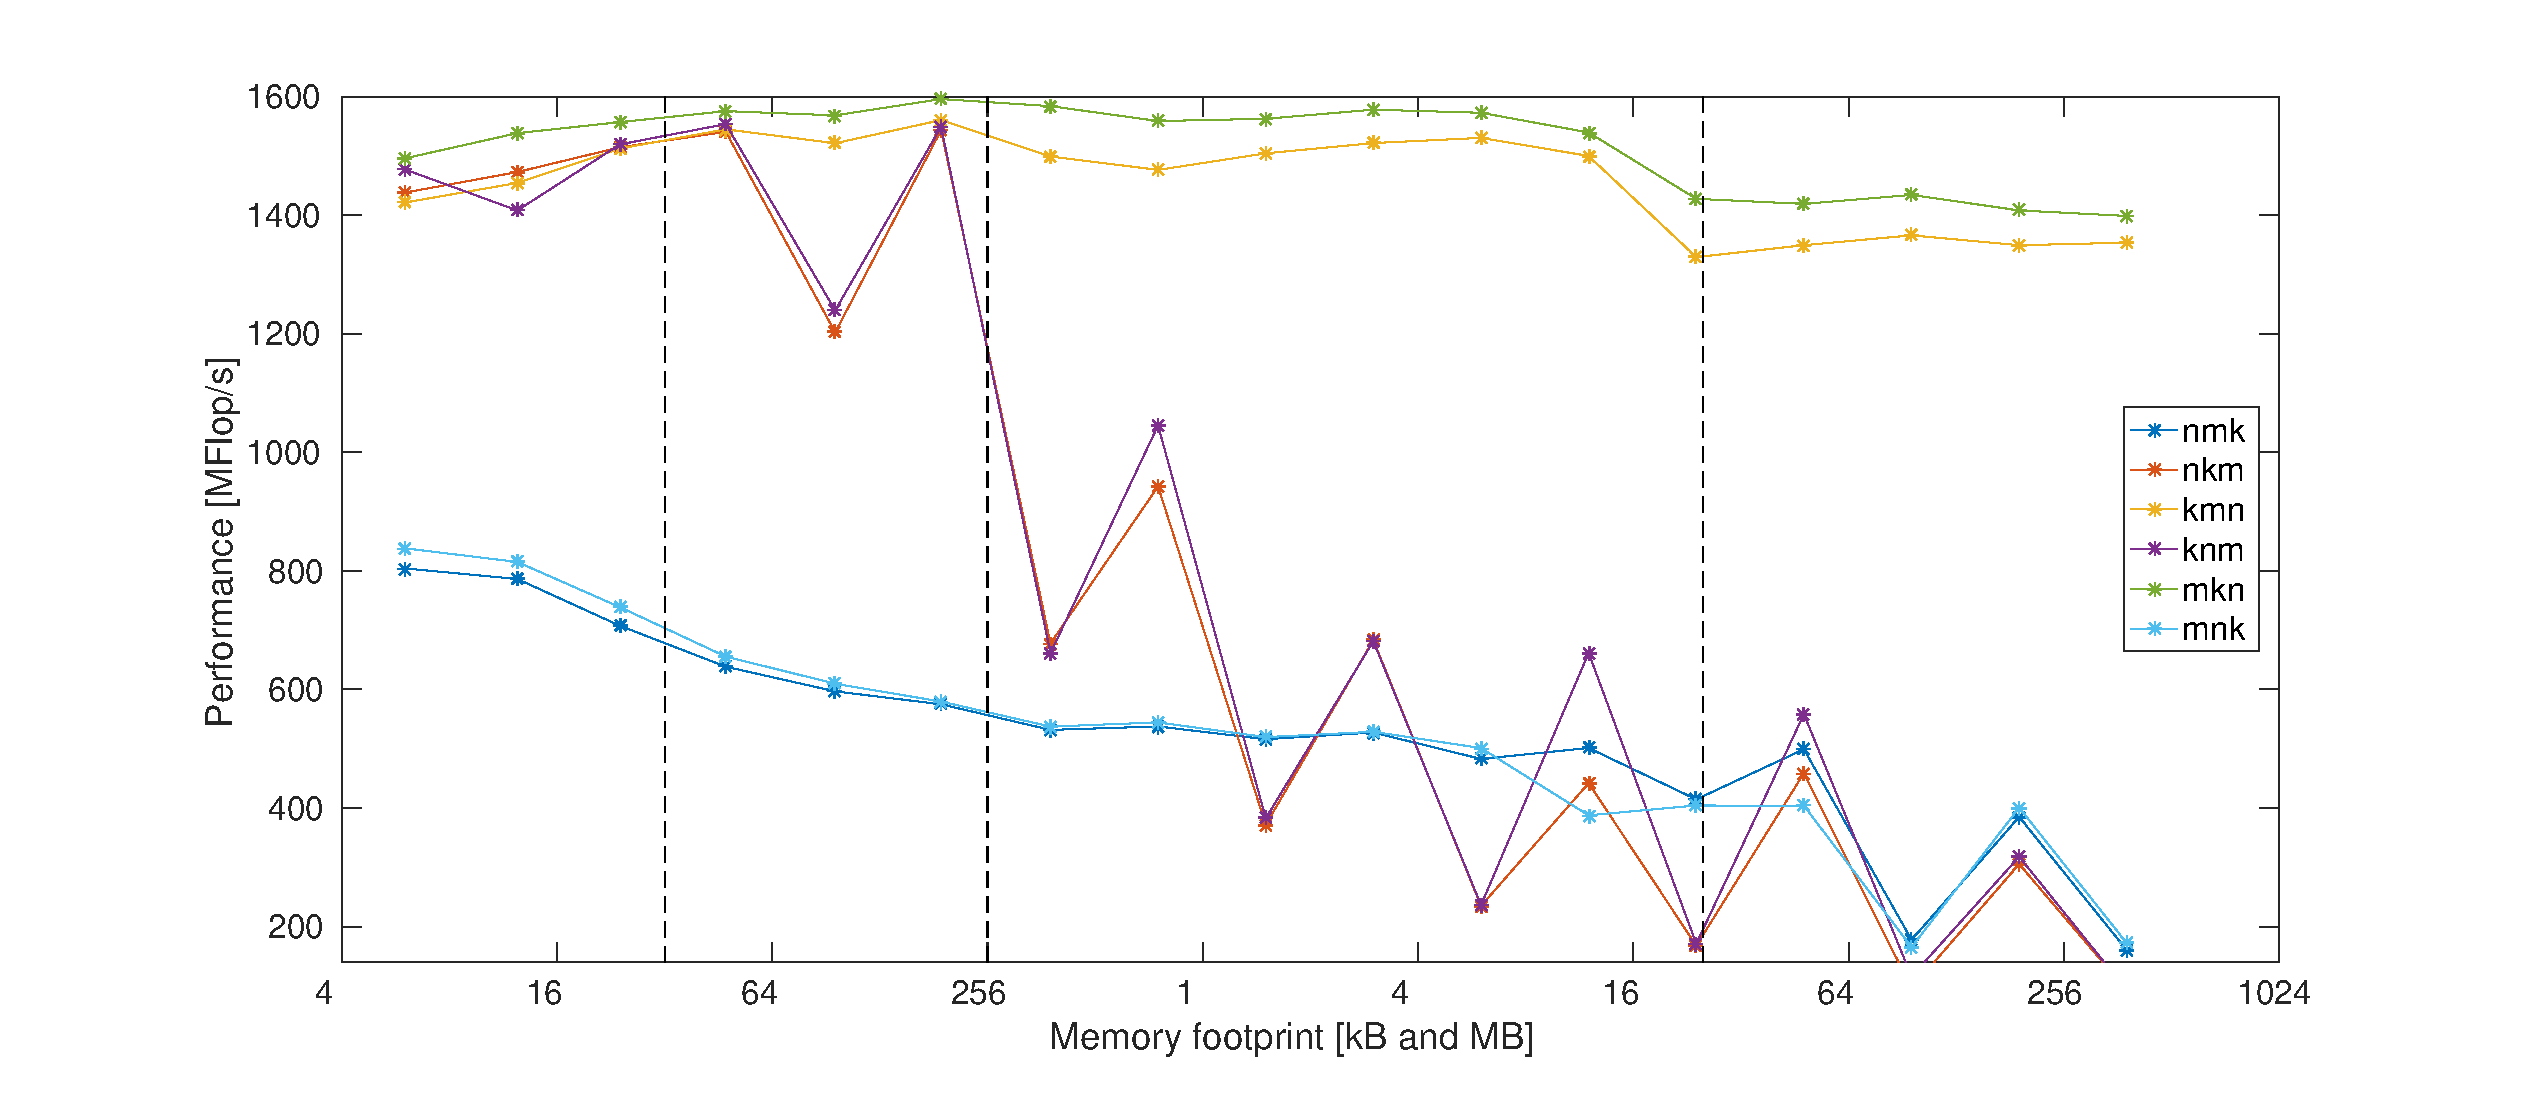
\includegraphics[width = 1.1\textwidth]{fig/permGraph_fast.eps}
\caption{This is a caption}
\label{fig:comp1}
\end{figure}

\subsubsection{Analyzer Tool}
We expect better-performing permutations to have less cache misses.   To validate our hypotheses regarding cache hits we conducted a profiling experiment. That is, we fixed the matrix dimension size to 1000 which corresponds to ~24MB memory footprint and ran each of the six permutations with and without compiler optimizations (with and without -fast). The results were collected and viewed using Oracle Solaris Studio Performance Analyzer. To be able to make direct comparisons, we set the minimum runtime to zero and max iterations to one. This way each permutation is run for a single iteration and we can compare cache hits in absolute terms. To directly compare, the relative hit ratio is computed for each permutation for both compiler settings and for both the L1d and L2d cache. \\
Table \ref{tab:tab1} shows the various hit ratios for the different permutations. It is clear, that both mkn and kmn has the fewest cache misses in the in L1 for both with and without fast. The hit ratios are worse in the L2 cache for the good performing mkn and kmn functions, but this is most likely due to the very few hits in that cache, since more of the L2 cache is used due to the fact of the faster computations. It is likewise found that nmk and mnk also perform averagely regarding the cache misses, which is also apparent in the memory foodprint since they are fluctuating between the bottom perfoming knm and nkm permutations and the top performing permutations of the mkn and kmn.


\begin{table}[h!]
\centering
\caption{Displaying L1 and L2 cache hit ratio for the various permutations for a 1000x1000 matrix.}
\label{Table:nat}
\begin{tabular}{|l|l|l||l|l|l|}
		\hline
 & No compiler optimization & & With -fast & \\ \hline
 & L1 hit ratio & L2 hit ratio & L1 hit ratio & L2 hit ratio \\ \hline
mkn & 99.98\%& 75.96\% & 99.94\% & 0 hits  \\  \hline
nkm & 90.22\% & 93.18\% &62.78\% & 93.53\% \\ \hline
nmk & 95.19\% & 99.69\% &84.38\% & 87.60\%   \\ \hline
mnk & 99.49\% & 87.43\% &84.46\% & 99.39\%  \\ \hline
kmn & 99.97\% & 61.24\% &99.94\% & 75.96\%  \\ \hline
knm & 90.20\% & 93.43\% &62.94\% & 93.08\%  \\ \hline
\end{tabular}
\end{table}

Since there were no hits in L2 for the mkn permutation, we performed a computation for a 2000x2000 matrix, just to provide the whole picture. Here the L1 ratio is found to be 99.91\% and 86.67\% for the L2 cache.

\subsection{Loop Blocking}

Loop blocking is a technique to improve the memory access and data re-use, and thereby reduce the cache misses. To perform this, the matrices is essentially cut into smaller blocks, which are then solved, where more of the information can be reused, since it is already available in the cache. By implementing loop blocking, we intend to compare the performance of the new blocked loop function with the best performing permutation, which is mkn. The function prototype is almost identical to the earlier used with the new addition, that it takes a specified integer bs as an argument.

\begin{lstlisting}[language=C++, caption=Function Prototype]
void matmult_blk(int m, int n, int k, double ** A, double ** B, double ** C, int bs)
\end{lstlisting}

To implement the blocking itself for arbitrarily sized matrices, we introduce 3 blocking size variables in the loop for each dimension. Since the blocking is performed for each dimension, we need six nested loops. The first three are the blocking loops to increases in increments of the blocking size. These include an if conditional, in the case, when the specific dimension is not dividable by the block variable. In the last run of the loop, there may be a case where the blocking size is actually bigger than the missing number of loop variables (dimension size - loop variable), in which case the bs variable is set equal to the number of missing rowx/columns for that dimension. This secures that no segmentation error occur.\\

The three inner loops basically runs over the according block sizes for the three dimension variables.

\begin{lstlisting}[language=C++, caption=Function Prototype]
int bsi=bs;
int bsj=bs;
int bsl=bs;

for(int i1 = 0; i1 < m;i1+=bsi){
	if(m-i1 < bs) {bsi=m-i1;
	}
	for(int l1 = 0; l1 < k;l1+=bsl){
		if(k-l1 < bs) {bsl=k-l1;
		}
		for(int j1 = 0; j1 < n;j1+=bsj){
			if(n-j1 < bs) {bsj=n-j1;
			}
			for(int i2 = 0; i2 < bsi; i2++){	
				for(int l2 = 0; l2 < bsl;l2++){	
					for(int j2 = 0; j2 < bsj; j2++){	
							C[i1+i2][j1+j2] += A[i1+i2][l1+l2]*B[l1+l2][j1+j2];
					}
				}
			}
		}
	}
}
\end{lstlisting}

It would also be easy to implement different initial block sizes to experiment with different block dimensions and structures, i.e. a rectangle, but this is however not researched in our report. 


\section{Conclusion}
We have implemented 6 functions all computing a matrix matrix product, and each having a different permutation of loop orders. Using different compiler optimizations, the best one was found to be mkn, topping at $\sim 1600$ MFlop/s, opposed to the DGEMM library function which tops at $\sim 22000$ MFlop/s. Cache hits and misses were analyzed to highlight the difference in performance between the permutations, and the analysis showed that the quickest functions has the highest hit-to-miss-ratio as expected. Finally, blocking was implemented as an attempt to better the performance degradation from the memory footprint exceeding the L3 cache size. The implementation was successful, but performance-wise, it only showed a minor improvement as opposed to the best non-blocked version. This is partly due to the Sun Studio compiler doing a great job at prefetching. However, we expect that the blocked version will be better than the non-blocked version for matrices larger than the one tested here.
\end{document}
